\section{Calculating Forward Rates}\label{calculating-forward-rates}

Last week we wrote a function called \texttt{df} for calculating a
discount factor at any date, given a set of discount factors each
relative to a corresponding pillar date, using log-linear interpolation.
Now we want a function to compute forward rates.

The formula to calculate the forward rates can be found exploiting the
property that investing at rate \(r_1\) for the period \((0, T_1)\) and
then \emph{reinvesting} at rate \(r_{1,2}\) for the time period
\((T_1, T_2)\) is equivalent to invest at rate \(r_2\) for the time
period \((0, T_2)\) (i.e.~no arbitrage condition, two investors
shouldn't be able to earn money from arbitraging between different
interest periods). That said:

\[(1+r_1 T_1)(1+r_{1,2}(T_2 - T_1)) = 1 + r_2 T_2\]

Solving for \(r_{1,2}\) leads to

\[F(T_1, T_2) = r_{1,2} = \frac{1}{T_2-T_1}\Big(\frac{D(T_1)}{D(T_2)} - 1 \Big)~~~~\textrm{(where $D{(T_i)}=\frac{1}{1+r_iT_{i}}$)}\]

    \begin{Verbatim}[commandchars=\\\{\}]
{\color{incolor}In [{\color{incolor} }]:} \PY{k+kn}{from} \PY{n+nn}{datetime} \PY{k}{import} \PY{n}{date}
        \PY{k+kn}{import} \PY{n+nn}{numpy}\PY{o}{,} \PY{n+nn}{math}
        
        \PY{n}{today\PYZus{}date} \PY{o}{=} \PY{n}{date} \PY{p}{(}\PY{l+m+mi}{2019}\PY{p}{,} \PY{l+m+mi}{1}\PY{p}{,} \PY{l+m+mi}{1}\PY{p}{)}
        
        \PY{n}{pillar\PYZus{}dates} \PY{o}{=} \PY{p}{[}\PY{n}{date}\PY{p}{(}\PY{l+m+mi}{2019} \PY{p}{,} \PY{l+m+mi}{1} \PY{p}{,}\PY{l+m+mi}{1}\PY{p}{)}\PY{p}{,} 
                        \PY{n}{date}\PY{p}{(}\PY{l+m+mi}{2020}\PY{p}{,} \PY{l+m+mi}{1}\PY{p}{,} \PY{l+m+mi}{1}\PY{p}{)}\PY{p}{,} 
                        \PY{n}{date}\PY{p}{(}\PY{l+m+mi}{2021}\PY{p}{,} \PY{l+m+mi}{10} \PY{p}{,}\PY{l+m+mi}{1}\PY{p}{)}\PY{p}{]}
        \PY{n}{discount\PYZus{}factors} \PY{o}{=} \PY{p}{[}\PY{l+m+mf}{1.0}\PY{p}{,} \PY{l+m+mf}{0.97}\PY{p}{,} \PY{l+m+mf}{0.72}\PY{p}{]}
        
        \PY{k}{def} \PY{n+nf}{df}\PY{p}{(}\PY{n}{d}\PY{p}{)}\PY{p}{:}
            \PY{n}{log\PYZus{}discount\PYZus{}factors} \PY{o}{=} \PY{p}{[}\PY{n}{math}\PY{o}{.}\PY{n}{log}\PY{p}{(}\PY{n}{discount\PYZus{}factor}\PY{p}{)} \PYZbs{}
                                    \PY{k}{for} \PY{n}{discount\PYZus{}factor} \PY{o+ow}{in} \PY{n}{discount\PYZus{}factors}\PY{p}{]}
            \PY{n}{pillar\PYZus{}days} \PY{o}{=} \PY{p}{[}\PY{p}{(}\PY{n}{pillar\PYZus{}date} \PY{o}{\PYZhy{}} \PY{n}{today\PYZus{}date}\PY{p}{)}\PY{o}{.}\PY{n}{days} \PYZbs{}
                           \PY{k}{for} \PY{n}{pillar\PYZus{}date} \PY{o+ow}{in} \PY{n}{pillar\PYZus{}dates}\PY{p}{]}
            \PY{n}{d\PYZus{}days} \PY{o}{=} \PY{p}{(}\PY{n}{d} \PY{o}{\PYZhy{}} \PY{n}{today\PYZus{}date}\PY{p}{)}\PY{o}{.}\PY{n}{days}
            \PY{n}{interpolated\PYZus{}log\PYZus{}discount\PYZus{}factor} \PY{o}{=} \PYZbs{}
                \PY{n}{numpy}\PY{o}{.}\PY{n}{interp}\PY{p}{(}\PY{n}{d\PYZus{}days}\PY{p}{,} \PY{n}{pillar\PYZus{}days}\PY{p}{,} \PY{n}{log\PYZus{}discount\PYZus{}factors}\PY{p}{)}
            
            \PY{k}{return} \PY{n}{math}\PY{o}{.}\PY{n}{exp}\PY{p}{(}\PY{n}{interpolated\PYZus{}log\PYZus{}discount\PYZus{}factor}\PY{p}{)}
        
        \PY{k}{def} \PY{n+nf}{forward\PYZus{}rate}\PY{p}{(}\PY{n}{t1}\PY{p}{,} \PY{n}{t2}\PY{p}{)}\PY{p}{:}
            \PY{k}{return} \PY{l+m+mf}{365.0}\PY{o}{/}\PY{p}{(}\PY{n}{t2}\PY{o}{\PYZhy{}}\PY{n}{t1}\PY{p}{)}\PY{o}{.}\PY{n}{days} \PY{o}{*} \PY{p}{(}\PY{n}{df}\PY{p}{(}\PY{n}{t1}\PY{p}{)} \PY{o}{/} \PY{n}{df}\PY{p}{(}\PY{n}{t2}\PY{p}{)} \PY{o}{\PYZhy{}} \PY{l+m+mi}{1}\PY{p}{)}
        
        \PY{n}{forward\PYZus{}rate}\PY{p}{(}\PY{n}{date}\PY{p}{(}\PY{l+m+mi}{2019}\PY{p}{,} \PY{l+m+mi}{2}\PY{p}{,} \PY{l+m+mi}{1}\PY{p}{)}\PY{p}{,} \PY{n}{date}\PY{p}{(}\PY{l+m+mi}{2019}\PY{p}{,} \PY{l+m+mi}{8}\PY{p}{,} \PY{l+m+mi}{1}\PY{p}{)}\PY{p}{)}
\end{Verbatim}

\hypertarget{financial-crisis}{%
\subsection{2008 Financial Crisis}\label{financial-crisis}}

Looking at the historical series of the Euribor (6M) rate versus the
Eonia Overnight Indexed Swap (OIS-6M) rate over the time interval
2006-2011 it becomes apparent how before August 2007 the two rates
display strictly overlapping trends differing of no more than 6 bps.

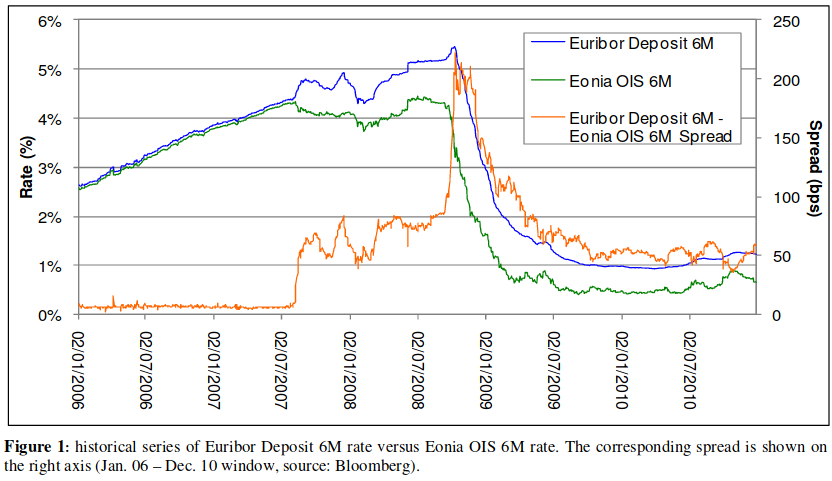
\includegraphics{credit_crunch.png}

In August 2007 however we observe a sudden increase of the Euribor rate
and a simultaneous decrease of the OIS rate that leads to the explosion
of the corresponding basis spread, touching the peak of 222 bps in
October 2008, when Lehman Brothers filed for bankruptcy protection.
Successively the basis has sensibly reduced and stabilized between 40
bps and 60 bps (notice that the pre-crisis level has never been
recovered). The same effect is observed for other similar couples,
e.g.~Euribor 3M vs OIS 3M.

The reason of the abrupt divergence between the Euribor and OIS rates
can be explained by considering both the monetary policy decisions
adopted by international authorities in response to the financial
turmoil, and the impact of the credit crunch on the credit and liquidity
risk perception of the market, coupled with the different financial
meaning and dynamics of these rates.

\begin{itemize}
\tightlist
\item
  The Euribor rate is the reference rate for over-the-counter (OTC)
  transactions in the Euro area. It is defined as ``the rate at which
  Euro interbank Deposits are being offered within the EMU zone by one
  prime bank to another at 11:00 a.m. Brussels time''. The rate fixings
  for a strip of 15 maturities, ranging from one day to one year, are
  constructed as the average of the rates submitted (excluding the
  highest and lowest 15\% tails) by a panel of banks 42 banks, selected
  among the EU banks with the highest volume of business in the Euro
  zone money markets, plus some large international bank from non-EU
  countries with important euro zone operations. \textbf{Thus, Euribor
  rates reflect the average cost of funding of banks in the interbank
  market at each given maturity. During the crisis the solvency and
  solidity of the whole financial sector was brought into question and
  the credit and liquidity risk and premia associated to interbank
  counterparties sharply increased.} The Euribor rates immediately
  reflected these dynamics and raise to their highest values over more
  than 10 years. As seen in the plot above, the Euribor 6M rate suddenly
  increased on August 2007 and reached 5.49\% on 10th October 2008.
\item
  The Eonia rate is the reference rate for overnight OTC transactions in
  the Euro area. It is constructed as the average rate of the overnight
  transactions (one day maturity deposits) executed during a given
  business day by a panel of banks on the interbank money market,
  weighted with the corresponding transaction volumes. \textbf{The Eonia
  Contribution Panel coincides with the Euribor Contribution Panel, thus
  Eonia rate includes information on the short term (overnight)
  liquidity expectations of banks in the Euro money market. It is also
  used by the European Central Bank (ECB) as a method of effecting and
  observing the transmission of its monetary policy actions. During the
  crisis the central banks were mainly concerned about restabilising the
  level of liquidity in the market, thus they reduced the level of the
  official rates.} Furthermore, the daily tenor of the Eonia rate makes
  negligible the credit and liquidity risks reflected on it: for this
  reason the OIS rates are considered the best proxies available in the
  market for the risk-free rate.
\end{itemize}

As a practial result, after the 2008 financial crisis, it is not
possible anymore to use a single discount curve to correctly price
forward rates of all tenors. For example, if we want to calculate the
net present value of a forward 6-month libor coupon, we need to
simultaneously use two different discount curves:

\begin{itemize}
\tightlist
\item
  the 6-month libor curve for determining the forward rate
\item
  the EONIA curve for discounting the expected cash flow
\end{itemize}

Essentially we are now going to explore how to implement the following
calculation:

\[\mathrm{NPV} = D_{\mathrm{EONIA}}(T_1) \times \frac{1}{T_2-T_1}\Big(\frac{D_{\mathrm{LIBOR}}(T_1)}{D_{\mathrm{LIBOR}}(T_2)} - 1 \Big)\]


However, as we have seen, Python allows you to represent collections of
objects with dictionaries. A clear improvement could be, instead of
passing a long list of data parameters to each function call, to group
the datasets into dictionaries, and then pass those to the function.
    This design pattern, i.e.~using dictionaries to group together data, and
then having functions operate on those dictionaries, perhaps with a few
additional parameters, is so useful that Python (and many other
programming languages) have a built-in feature that allows you to do
this conveniently: \textbf{classes}.
So now that we have an idea of what a class is, try to write a
\texttt{DiscountCurve} class which contains the pillar dates and pillar
discount factors as attributes and which has methods for calculating the
discount factor and forward rate at arbitrary dates.

\hypertarget{solution}{%
\paragraph{Solution:}\label{solution}}

    \begin{Verbatim}[commandchars=\\\{\}]
{\color{incolor}In [{\color{incolor}4}]:} \PY{k+kn}{import} \PY{n+nn}{math}
        \PY{k+kn}{import} \PY{n+nn}{numpy}
        \PY{k+kn}{from} \PY{n+nn}{datetime} \PY{k}{import} \PY{n}{date}
        
        \PY{k}{class} \PY{n+nc}{DiscountCurve}\PY{p}{:}
        
            \PY{c+c1}{\PYZsh{} the special \PYZus{}\PYZus{}init\PYZus{}\PYZus{} method defines }
            \PY{c+c1}{\PYZsh{} how to construct instances of the class}
            \PY{k}{def} \PY{n+nf}{\PYZus{}\PYZus{}init\PYZus{}\PYZus{}}\PY{p}{(}\PY{n+nb+bp}{self}\PY{p}{,} \PY{n}{today}\PY{p}{,} \PY{n}{pillar\PYZus{}dates}\PY{p}{,} \PY{n}{discount\PYZus{}factors}\PY{p}{)}\PY{p}{:}
                \PY{c+c1}{\PYZsh{} we just store the arguments as attributes of the instance}
                \PY{n+nb+bp}{self}\PY{o}{.}\PY{n}{today} \PY{o}{=} \PY{n}{today}
                \PY{n+nb+bp}{self}\PY{o}{.}\PY{n}{pillar\PYZus{}dates} \PY{o}{=} \PY{n}{pillar\PYZus{}dates}
                \PY{n+nb+bp}{self}\PY{o}{.}\PY{n}{discount\PYZus{}factors} \PY{o}{=} \PY{n}{discount\PYZus{}factors}
        
            \PY{c+c1}{\PYZsh{} calculates a discount factor at an arbitrary }
            \PY{c+c1}{\PYZsh{}value date using the data stored in the instance}
            \PY{k}{def} \PY{n+nf}{df}\PY{p}{(}\PY{n+nb+bp}{self}\PY{p}{,} \PY{n}{d}\PY{p}{)}\PY{p}{:}
                \PY{c+c1}{\PYZsh{} these remain local variables, }
                \PY{c+c1}{\PYZsh{} i.e. they are only available within the function.}
                \PY{c+c1}{\PYZsh{} to read (or write) instance attributes, }
                \PY{c+c1}{\PYZsh{} you always need to use the self. syntax}
                \PY{n}{log\PYZus{}discount\PYZus{}factors} \PY{o}{=} \PYZbs{}
                  \PY{p}{[}\PY{n}{math}\PY{o}{.}\PY{n}{log}\PY{p}{(}\PY{n}{discount\PYZus{}factor}\PY{p}{)} 
                   \PY{k}{for} \PY{n}{discount\PYZus{}factor} \PY{o+ow}{in} \PY{n+nb+bp}{self}\PY{o}{.}\PY{n}{discount\PYZus{}factors}\PY{p}{]}
                \PY{n}{pillar\PYZus{}days} \PY{o}{=} \PY{p}{[}\PY{p}{(}\PY{n}{pillar\PYZus{}date} \PY{o}{\PYZhy{}} \PY{n+nb+bp}{self}\PY{o}{.}\PY{n}{today}\PY{p}{)}\PY{o}{.}\PY{n}{days} 
                               \PY{k}{for} \PY{n}{pillar\PYZus{}date} \PY{o+ow}{in} \PY{n+nb+bp}{self}\PY{o}{.}\PY{n}{pillar\PYZus{}dates}\PY{p}{]}
                \PY{n}{d\PYZus{}days} \PY{o}{=} \PY{p}{(}\PY{n}{d} \PY{o}{\PYZhy{}} \PY{n+nb+bp}{self}\PY{o}{.}\PY{n}{today}\PY{p}{)}\PY{o}{.}\PY{n}{days}
                \PY{n}{interpolated\PYZus{}log\PYZus{}discount\PYZus{}factor} \PY{o}{=} \PYZbs{}
                    \PY{n}{numpy}\PY{o}{.}\PY{n}{interp}\PY{p}{(}\PY{n}{d\PYZus{}days}\PY{p}{,} \PY{n}{pillar\PYZus{}days}\PY{p}{,} \PY{n}{log\PYZus{}discount\PYZus{}factors}\PY{p}{)}
                \PY{k}{return} \PY{n}{math}\PY{o}{.}\PY{n}{exp}\PY{p}{(}\PY{n}{interpolated\PYZus{}log\PYZus{}discount\PYZus{}factor}\PY{p}{)}
        
            \PY{c+c1}{\PYZsh{} calculates a forward libor rate based on the discount }
            \PY{c+c1}{\PYZsh{} curve data stored in the instance}
            \PY{k}{def} \PY{n+nf}{forward\PYZus{}rate}\PY{p}{(}\PY{n+nb+bp}{self}\PY{p}{,} \PY{n}{d1}\PY{p}{,} \PY{n}{d2}\PY{p}{)}\PY{p}{:}
                \PY{c+c1}{\PYZsh{} we use the df method of the current instance to calculate}
                \PY{c+c1}{\PYZsh{} the forward rate}
                \PY{k}{return} \PY{p}{(}\PY{n+nb+bp}{self}\PY{o}{.}\PY{n}{df}\PY{p}{(}\PY{n}{d1}\PY{p}{)} \PY{o}{/} \PY{n+nb+bp}{self}\PY{o}{.}\PY{n}{df}\PY{p}{(}\PY{n}{d2}\PY{p}{)} \PY{o}{\PYZhy{}} \PY{l+m+mf}{1.0}\PY{p}{)} \PY{o}{*} \PYZbs{}
                        \PY{p}{(}\PY{l+m+mf}{365.0} \PY{o}{/} \PY{p}{(}\PY{p}{(}\PY{n}{d2} \PY{o}{\PYZhy{}} \PY{n}{d1}\PY{p}{)}\PY{o}{.}\PY{n}{days}\PY{p}{)}\PY{p}{)}
\end{Verbatim}

    \begin{Verbatim}[commandchars=\\\{\}]
{\color{incolor}In [{\color{incolor}5}]:} \PY{c+c1}{\PYZsh{} build the EONIA curve object}
        \PY{c+c1}{\PYZsh{} n.b. here we use the \PYZsq{}parameter=argument\PYZsq{} syntax }
        \PY{c+c1}{\PYZsh{} (today=..., pillar\PYZus{}dates=...)}
        \PY{c+c1}{\PYZsh{} just so it\PYZsq{}s really clear what we\PYZsq{}re doing - it\PYZsq{}s not necessary, }
        \PY{c+c1}{\PYZsh{} it\PYZsq{}s only for clarity}
        \PY{n}{eonia\PYZus{}curve} \PY{o}{=} \PY{n}{DiscountCurve}\PY{p}{(}\PY{n}{today}\PY{o}{=}\PY{n}{date}\PY{p}{(}\PY{l+m+mi}{2019}\PY{p}{,} \PY{l+m+mi}{10}\PY{p}{,} \PY{l+m+mi}{1}\PY{p}{)}\PY{p}{,}
                                    \PY{n}{pillar\PYZus{}dates}\PY{o}{=}\PY{p}{[}\PY{n}{date}\PY{p}{(}\PY{l+m+mi}{2019}\PY{p}{,} \PY{l+m+mi}{10}\PY{p}{,} \PY{l+m+mi}{1}\PY{p}{)}\PY{p}{,} 
                                                  \PY{n}{date}\PY{p}{(}\PY{l+m+mi}{2020}\PY{p}{,} \PY{l+m+mi}{10}\PY{p}{,} \PY{l+m+mi}{1}\PY{p}{)}\PY{p}{,} 
                                                  \PY{n}{date}\PY{p}{(}\PY{l+m+mi}{2021}\PY{p}{,} \PY{l+m+mi}{10}\PY{p}{,} \PY{l+m+mi}{1}\PY{p}{)}\PY{p}{]}\PY{p}{,}
                                    \PY{n}{discount\PYZus{}factors}\PY{o}{=}\PY{p}{[}\PY{l+m+mf}{1.0}\PY{p}{,} \PY{l+m+mf}{0.95}\PY{p}{,} \PY{l+m+mf}{0.8}\PY{p}{]}\PY{p}{)}
        
        \PY{c+c1}{\PYZsh{} build the Libor curve object}
        \PY{n}{libor\PYZus{}curve} \PY{o}{=} \PY{n}{DiscountCurve}\PY{p}{(}\PY{n}{today}\PY{o}{=}\PY{n}{date}\PY{p}{(}\PY{l+m+mi}{2019}\PY{p}{,} \PY{l+m+mi}{10}\PY{p}{,} \PY{l+m+mi}{1}\PY{p}{)}\PY{p}{,}
                                    \PY{n}{pillar\PYZus{}dates}\PY{o}{=}\PY{p}{[}\PY{n}{date}\PY{p}{(}\PY{l+m+mi}{2019}\PY{p}{,} \PY{l+m+mi}{10}\PY{p}{,} \PY{l+m+mi}{1}\PY{p}{)}\PY{p}{,} 
                                                  \PY{n}{date}\PY{p}{(}\PY{l+m+mi}{2020}\PY{p}{,} \PY{l+m+mi}{4}\PY{p}{,} \PY{l+m+mi}{1}\PY{p}{)}\PY{p}{,} 
                                                  \PY{n}{date}\PY{p}{(}\PY{l+m+mi}{2020}\PY{p}{,} \PY{l+m+mi}{10}\PY{p}{,} \PY{l+m+mi}{1}\PY{p}{)}\PY{p}{]}\PY{p}{,}
                                    \PY{n}{discount\PYZus{}factors}\PY{o}{=}\PY{p}{[}\PY{l+m+mf}{1.0}\PY{p}{,} \PY{l+m+mf}{0.98}\PY{p}{,} \PY{l+m+mf}{0.82}\PY{p}{]}\PY{p}{)}
        
        \PY{c+c1}{\PYZsh{} Let\PYZsq{}s compute the discount factor of the two curves}
        \PY{c+c1}{\PYZsh{} on the 2020\PYZhy{}5\PYZhy{}1}
        \PY{n+nb}{print} \PY{p}{(}\PY{n}{eonia\PYZus{}curve}\PY{o}{.}\PY{n}{df}\PY{p}{(}\PY{n}{date}\PY{p}{(}\PY{l+m+mi}{2020}\PY{p}{,} \PY{l+m+mi}{5}\PY{p}{,} \PY{l+m+mi}{1}\PY{p}{)}\PY{p}{)}\PY{p}{)}
        \PY{n+nb}{print} \PY{p}{(}\PY{n}{libor\PYZus{}curve}\PY{o}{.}\PY{n}{df}\PY{p}{(}\PY{n}{date}\PY{p}{(}\PY{l+m+mi}{2020}\PY{p}{,} \PY{l+m+mi}{5}\PY{p}{,} \PY{l+m+mi}{1}\PY{p}{)}\PY{p}{)}\PY{p}{)}
\end{Verbatim}

    \begin{Verbatim}[commandchars=\\\{\}]
0.9705901255781632
0.9517777485424973

    \end{Verbatim}

    \begin{Verbatim}[commandchars=\\\{\}]
{\color{incolor}In [{\color{incolor}6}]:} \PY{c+c1}{\PYZsh{} Let\PYZsq{}s compute now the 6m forward rate at 1\PYZhy{}4\PYZhy{}2020}
        \PY{n+nb}{print} \PY{p}{(}\PY{n}{eonia\PYZus{}curve}\PY{o}{.}\PY{n}{forward\PYZus{}rate}\PY{p}{(}\PY{n}{date}\PY{p}{(}\PY{l+m+mi}{2019}\PY{p}{,} \PY{l+m+mi}{10}\PY{p}{,} \PY{l+m+mi}{1}\PY{p}{)}\PY{p}{,} 
                                         \PY{n}{date}\PY{p}{(}\PY{l+m+mi}{2020}\PY{p}{,} \PY{l+m+mi}{10}\PY{p}{,} \PY{l+m+mi}{1}\PY{p}{)}\PY{p}{)}\PY{p}{)}
        
        \PY{n+nb}{print} \PY{p}{(}\PY{n}{libor\PYZus{}curve}\PY{o}{.}\PY{n}{forward\PYZus{}rate}\PY{p}{(}\PY{n}{date}\PY{p}{(}\PY{l+m+mi}{2020}\PY{p}{,} \PY{l+m+mi}{4}\PY{p}{,} \PY{l+m+mi}{1}\PY{p}{)}\PY{p}{,} 
                                         \PY{n}{date}\PY{p}{(}\PY{l+m+mi}{2020}\PY{p}{,} \PY{l+m+mi}{10}\PY{p}{,} \PY{l+m+mi}{1}\PY{p}{)}\PY{p}{)}\PY{p}{)}
\end{Verbatim}

    \begin{Verbatim}[commandchars=\\\{\}]
0.05248777681909687
0.3891776622684259

    \end{Verbatim}

    \begin{Verbatim}[commandchars=\\\{\}]
{\color{incolor}In [{\color{incolor}7}]:} \PY{c+c1}{\PYZsh{} Compute the NPV of the 6m forward libor coupon}
        \PY{n}{npv} \PY{o}{=} \PY{n}{eonia\PYZus{}curve}\PY{o}{.}\PY{n}{df}\PY{p}{(}\PY{n}{date}\PY{p}{(}\PY{l+m+mi}{2020}\PY{p}{,} \PY{l+m+mi}{4}\PY{p}{,} \PY{l+m+mi}{1}\PY{p}{)}\PY{p}{)} \PY{o}{*} \PYZbs{}
              \PY{n}{libor\PYZus{}curve}\PY{o}{.}\PY{n}{forward\PYZus{}rate}\PY{p}{(}\PY{n}{date}\PY{p}{(}\PY{l+m+mi}{2020}\PY{p}{,}\PY{l+m+mi}{4}\PY{p}{,} \PY{l+m+mi}{1}\PY{p}{)}\PY{p}{,} 
                                        \PY{n}{date}\PY{p}{(}\PY{l+m+mi}{2020}\PY{p}{,} \PY{l+m+mi}{10}\PY{p}{,} \PY{l+m+mi}{1}\PY{p}{)}\PY{p}{)}
        
        \PY{c+c1}{\PYZsh{} Compute it in the pre\PYZhy{}2008 way}
        \PY{n}{npv\PYZus{}pre\PYZus{}2008} \PY{o}{=} \PY{n}{libor\PYZus{}curve}\PY{o}{.}\PY{n}{df}\PY{p}{(}\PY{n}{date}\PY{p}{(}\PY{l+m+mi}{2020}\PY{p}{,} \PY{l+m+mi}{4}\PY{p}{,} \PY{l+m+mi}{1}\PY{p}{)}\PY{p}{)} \PY{o}{*} \PYZbs{}
                       \PY{n}{libor\PYZus{}curve}\PY{o}{.}\PY{n}{forward\PYZus{}rate}\PY{p}{(}\PY{n}{date}\PY{p}{(}\PY{l+m+mi}{2020}\PY{p}{,} \PY{l+m+mi}{4}\PY{p}{,} \PY{l+m+mi}{1}\PY{p}{)}\PY{p}{,} 
                                                 \PY{n}{date}\PY{p}{(}\PY{l+m+mi}{2020}\PY{p}{,} \PY{l+m+mi}{10}\PY{p}{,} \PY{l+m+mi}{1}\PY{p}{)}\PY{p}{)}
        \PY{n+nb}{print} \PY{p}{(}\PY{n}{npv}\PY{p}{)}
        \PY{n+nb}{print} \PY{p}{(}\PY{n}{npv\PYZus{}pre\PYZus{}2008}\PY{p}{)}
\end{Verbatim}

    \begin{Verbatim}[commandchars=\\\{\}]
0.37932346377238657
0.38139410902305737

    \end{Verbatim}

